\documentclass[a4paper]{article}
\usepackage[letterpaper, margin=1in]{geometry} % page format
\usepackage{listings} % this package is for including code
\usepackage{amsmath}  % this package is for math and matrices
\usepackage{amsfonts} % this package is for math fonts
\usepackage{hyperref} % for urls
\usepackage{dirtree}  % for directory trees
\usepackage{graphicx} % for figures
\usepackage{tikz}     % for special diagrams   -----------------
\usetikzlibrary{positioning,calc}
\tikzset{
  redondo/.style={
    draw=black,
    line width=1pt,
    rounded corners=3pt,
    minimum height=1.2em,
    text width=#1
  },
  punto/.style={
    circle,
    inner sep=0pt,
    text width=2.5mm,
    fill=gray!50!black
  },
  tresp/.pic={
    \node[punto] at (0.25,0) {};
    \node[punto] at (0.5,0) {};
    \node[punto] at (0.75,0) {};
  },
  trespg/.pic={
    \node[punto,fill=gray!90!black] at (0.25,0) {};
    \node[punto,fill=gray!90!black] at (0.5,0) {};
    \node[punto,fill=gray!90!black] at (0.75,0) {};
  },
  dosp/.pic={
    \node[punto] at (0.25,0) {};
    \node[punto] at (0.5,0) {};
  },
  unop/.pic={
    \node[punto] at (0.5,0) {};
  },
  cuadra/.style={
    fill=white,
    line width=0.1pt,
    minimum size=0.1pt
  },
  arr/.style={
    line width=1pt,
    draw=gray,
    ->,
    >=latex
  }  
}
%------------------------------- end of special diagrams



\title{A deep learning approach to sign language recognition using stacked 
autoencoders and neural networks}
\author{Pablo Rivas}
\date{Jan/24/17}

\begin{document}
\lstset{language=Python}

\maketitle

\section{Introduction}

Language is an essential part of being human as it enables us to communicate
with others. Some people have to develop additional means of communication
for different reasons. A popular alternative language is through signs. This
type of language is based on symbols or figures produced using the hands. 

Sign language recognition is a task that has been studied in the last few years
\cite{starner1998real}. We believe this is an important problem to address
because it directly affects the quality of life of people who need to
communicate using sign language. The task is to develop algorithms that can
recognize different signs in an alphabet and that can do so in an efficient
manner. Ideally, the methodologies should be fast to the point of enabling the 
near real-time processing of signs \cite{starner1997real}.

In this research we deal with the recognition of signs over the american sign
language (ASL). The proposed approach uses depth images of subjects making
different signs, building upon the work of B. Kang, et.al. in
\cite{kang2015real}. 

Typical approaches involve the using hidden Markov models
\cite{starner1997real}, and a combination of them with other discriminative
functions for feature extraction in multi-stage architectures
\cite{lichtenauer2008sign}. Other major alternatives included the exploration
of neural strategies combined with fuzzy systems \cite{al2001recognition}. For
a more detaile review of alternatives for generic hand gesture recognition we
can turn to the work in \cite{murthy2009review}.

However, with the dramatic attention that deep learning has gained recently 
in the machine learning and the immage processing for pattern recognition
communities, we are motivated to similarly explore this new algoritmic
alternative to see if it offers better solutions to open problems. Most
recently, the authors in \cite{kang2015real} have explored a deep learning
approach based on convolutional neural networks (CNNs) achieving outstanding
results. The research presented here also explores a novel deep learning
approach but based in autoencoders and neural networks. We will show that this
alternative approach achieves great performance and efficiency.

The rest of the paper is organized as follows. 


\section{Background and Related Work}

Recently, J. Nagi et.al. \cite{nagi2011max} studied a deep neural network
approach for recognizing six different hand gestures given to a robot. Using
CNNs the authors achieve a 96\% accuracy rate. Then, M. Van den Bergh et.al.
\cite{van2011combining} explored the idea of using depth-sensor imagery to
establish an algorithm for hand segmentation. The authors ultimately used this
to recognize six different hand gestures in 3D. They achieved a 99.54\%
recognition rate. Some of the key commonents of the overall architecture were
the usage of wavelets for image filtering and neural networks.

Moreover, B. Kang et.al. \cite{kang2015real} took advantage of the recent
success of CNNs for pattern recognition over images. They propose a system that
makes use of depth-sensor images to study further the problem of hand gesture
recognition. When recognizing signs within the same subject they averaged a 99.99\%
accuracy rate over five subjects. However, when recognizing signs across
different subjects, their accuracy rate droped to 83.58\%. 

Our research aims to further study the problem posed in \cite{kang2015real} of
increasing accuracy rates over different subjects. In the next section we
discuss the dataset used and propose a deep learning approach using
autoencoders and a neural network. 


\section{Methodology}

\subsection{Data}

This research focuses in the ASL as a case study \cite{baker1980american}. 
The ASL has 26 hand gestures 
corresponding to the letters in the English alphabet; it also contains 9 hand
gestures for every single number. Figure \ref{fig:asl} 
depicts the gestures pertaining to our study.

\begin{figure}
\centering
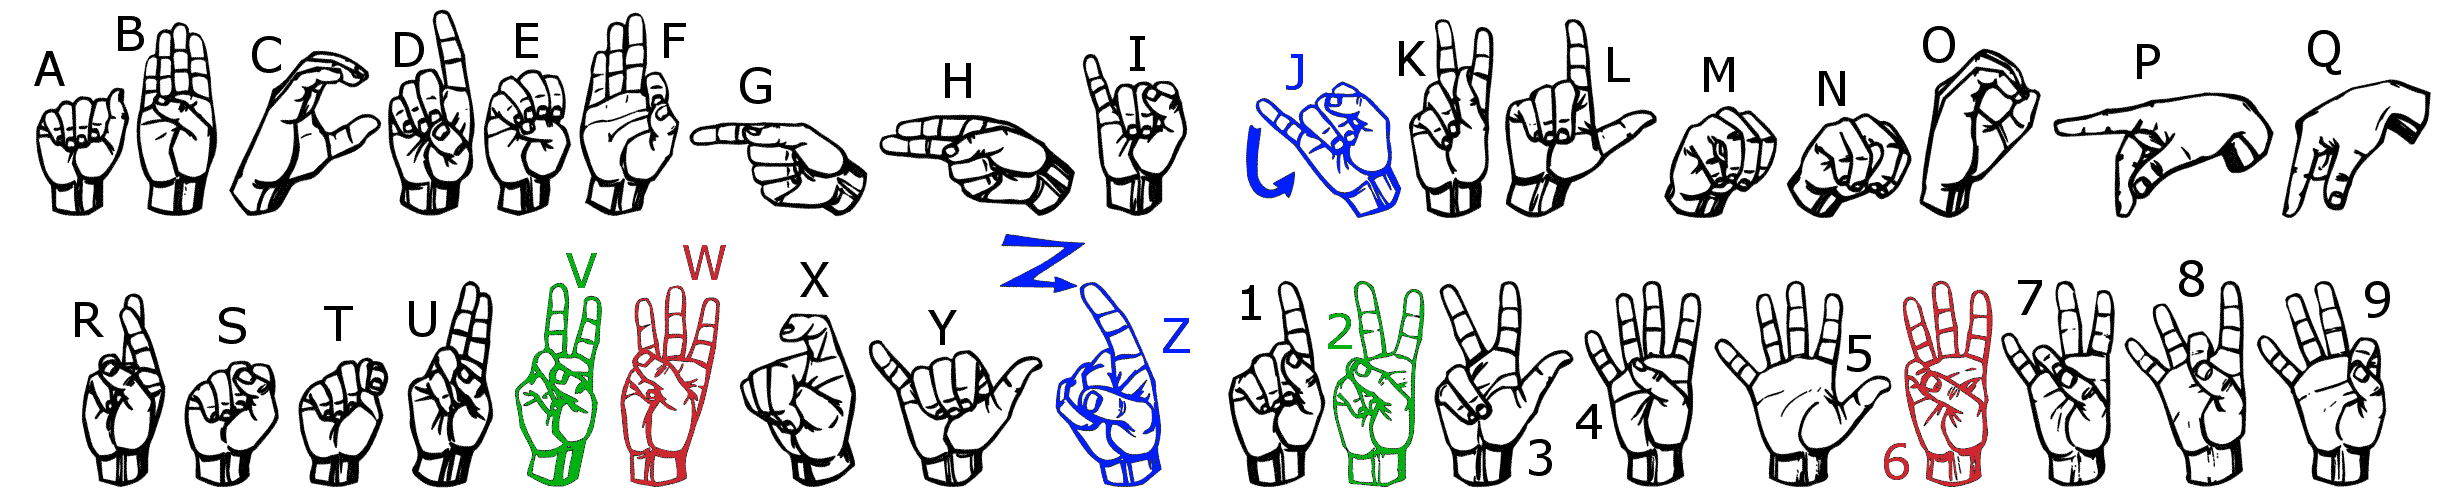
\includegraphics[width=\textwidth]{img/signs.eps}
\caption{The American Sign Language (ASL) displaying 26 signs corresponding to the
English alphabet (A to Z) and 9 signs for numbers (1 to 9).}
\label{fig:asl}
\end{figure}

We use the data provided in \cite{kang2015real} that was released in 2015. This
dataset consists of images acquired with a three-dimensional depth-sensor camera. 
There is a total of $31,000$ images available with a resolution of $256 \times
256$. The images correspond to already segmented dept-images that contain the
area of the hand. The authors use a rather simple algorithm to make the
segmentation based on the fact that in all depth images the hand is the closest
object with respect to the camera. 

Not all the 35 signs (26 letters and 9 numbers) 
were considered in this study. Some signs
were exluded and others considered jointly as follows.

The signs corresponding to J and Z clearly require a sequence of images rather
than a single instance, as can be seen in Figure \ref{fig:asl}. This goes
beyond the scope of this project; although the detection of signs from
live-video sequences is part of a bigger project, we will not address it in this
paper. For that reason these two signs were exluded.

The signs corresponding to V and 2, by observation, are nearly identical and
their distinction requires contextual information. Similarly, the signs for
letter W and number 6 require being interpreted in context. 
For this reason, these signs were considered as the same sign, leaving a total
of 31 signs.

There is a total of five different 
subjects and each subject produced 200 images of each
sign. This represents a total 1,000 images per sign and 31,000 images overall.
The images collected capture each subject making a hand gesture moving across
the horizontal axis and varying inclination of the hand gesture, as depicted in
Figure \ref{fig:sampN1}.

\begin{figure}
\centering
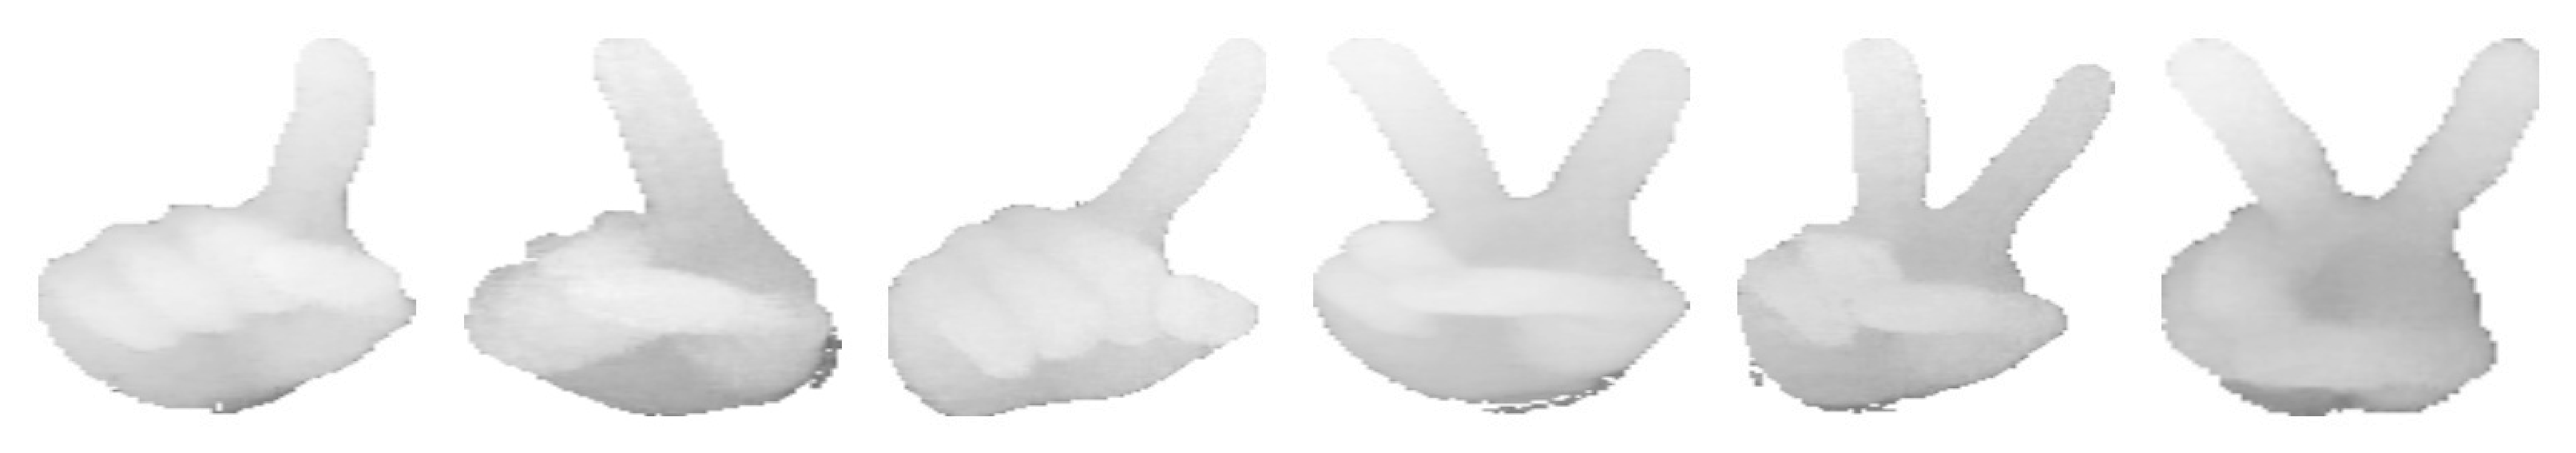
\includegraphics[width=\textwidth]{img/sampleNum1.eps}
\caption{Examples of ASL hand gestures corresponding to the number one and 
number two with variations in
the horizontal axis and its inclination with respect to a depth-sensor camera.}
\label{fig:sampN1}
\end{figure}


\subsection{Sparse Autoencoders}

A sparse autoencoder is usually categorized as a neural network with
unsupervised learning \cite{le2013building}. In a general sense an autoencoder
is trained to output an approximation of the input provided a deep architecture
of layered neurons that encode and decode based on the input stimuli. 
In our research we use a sparse autoencoder that specifically
minimizes a modified loss function based on the mean squared error. 

Let $\mathbf{x} \in \mathbb{R}^d$ be a $d$-dimensional input vector. Then the
loss function of the common sparse autoencoder is defined as follows:
\begin{align}
L=\frac{1}{N} \left\| \mathbf{x}_n - \mathbf{\hat{x}}_n  \right\|^2_2
+ \theta_w \frac{1}{2} \sum^L_{l=1} \left\| \mathbf{w}^l \right\|^2_2 +
\theta_s \sum^{M}_{m=1} KL \left( \theta_\alpha \left\| \bar{\alpha}_m \right. \right)
\label{eq:loss}
\end{align}
where $N$ is the total number of training samples; 
$\mathbf{\hat{x}}_n$ is the learned (or encoded) approximation of the
$n$-th input vector $\mathbf{x}_n$;
$\theta_w$ controls the sparsenes of the weights of the network, $\mathbf{w} \in
\mathbb{R}^d$;
$L$ denotes the number of layers in the deep network;
$\theta_s$ regulates the sparsity of the activation functions' output,
$\alpha$, in every neuron in the network;
$M$ is the total number of neurons in the deep network;
and $KL(\cdot)$ is the Kullback-Leibler divergence function 
\cite{joyce2011kullback} used to measure how
much the observed average activation of the $m$-th neuron, $\bar{\alpha}_m$,
actually deviates from the desired average output, $\theta_\alpha$.

The Kullback-Leibler divergence function can be defined as follows
\cite{olshausen1997sparse}: 
\begin{align}
\sum^M_{m=1} KL \left( \theta_\alpha \left\| \bar{\alpha}_m \right. \right) = 
\sum^M_{m=1} \theta_\alpha \log \left( \frac{\theta_\alpha}{\bar{\alpha}_m} \right)
+ (1 - \theta_\alpha) \log \left( \frac{1-\theta_\alpha}{1-\bar{\alpha}_m} \right)
\end{align}
where the average output of the $m$-th neuron, $\bar{\alpha}_m$, at the $l$-th
layer is given by
\begin{align}
\bar{\alpha}_m = \frac{1}{N} \sum^N_{n=1} \psi \left( \mathbf{w}^{(l)T}_m
\mathbf{x}_n + b^{(l)}_m \right)
\end{align}
where $\psi(\cdot)$ is the neuron's activation function, and
$b^{(l)}_m$ is the bias term for the $m$-th neuron at the $l$-th layer. 
In this research we specifically use logistic (sigmoid) activation functions,
$\psi(z) = 1/(1-e^{-z})$, for any given value of $z$. 

By observing the mathematical form of (\ref{eq:loss}), it is feasible to apply
an accelerated form of guided learning known as scaled conjugate gradient (SCG)
descent \cite{moller1993scaled}. SCG has proven to be a reliable and efficient
form of minimizing loss functions such as the one for the sparse autoencoder,
overcoming the shorcomings of a traditional conjugate gradient and
a back-propagation with gradient descents \cite{le2013building}. 


\subsection{Deep Learning Architecture}

Two stacked autoencoders are combined with a feedforward neural network in a
five-layer architecture, as shown in Figure \ref{fig:TrainingArchitecture}. 
\begin{figure}
\centering
\begin{tikzpicture}[node distance=1.5cm and 1.25cm]
\node[redondo=2cm,label={120:31 neural units}]
  (upper)
  {};
\pic at (upper.west) {dosp};
\pic at ([xshift=-0.75cm]upper.east) {unop};
\node[] 
  at ([xshift=4pt,yshift=-1pt]$ (upper.center) $ ) {$\ldots$};


\node[redondo=6.4cm,draw=gray,below=of upper,label={140:100 neural units}]
  (middleDec)
  {};
\pic at (middleDec.west) {trespg};
\pic at ([xshift=-1.85cm]middleDec) {trespg};
\pic at ([xshift=-2.58cm]middleDec) {trespg};
\pic at ([xshift=-1cm]middleDec.east) {trespg};
\node[] at ([xshift=4pt,yshift=-1pt]middleDec) {$\ldots$};



\node[redondo=3.3cm,below=of middleDec,label={140:50 neural units}]
  (middle)
  {};
\pic at (middle.west) {tresp};
\pic at ([xshift=-1.04cm]middle) {dosp};
\pic at ([xshift=-0.75cm]middle.east) {dosp};
\node[] at ([xshift=4pt,yshift=-1pt]middle) {$\ldots$};


\node[redondo=12cm,draw=gray,below=of middle,label={140:65536 neural units}]
  (lowerMiddleDec)
  {};
\pic at (lowerMiddleDec.west) {trespg};
\pic at ([xshift=-5.38cm]lowerMiddleDec) {trespg};
\pic at ([xshift=-4.65cm]lowerMiddleDec) {trespg};
\pic at ([xshift=-3.92cm]lowerMiddleDec) {trespg};
\pic at ([xshift=-3.19cm]lowerMiddleDec) {trespg};
\pic at ([xshift=-2.46cm]lowerMiddleDec) {trespg};
\pic at ([xshift=-1.73cm]lowerMiddleDec) {trespg};
\pic at ([xshift=-1.75cm]lowerMiddleDec.east) {trespg};
\pic at ([xshift=-1.00cm]lowerMiddleDec.east) {trespg};
\node[] at ([xshift=4pt,yshift=-1pt]lowerMiddleDec) {$\ldots$};


\node[redondo=6.4cm,below=of lowerMiddleDec,label={140:100 neural units}]
  (lowermiddle)
  {};
\pic at (lowermiddle.west) {tresp};
\pic at ([xshift=-1.85cm]lowermiddle) {tresp};
\pic at ([xshift=-2.58cm]lowermiddle) {tresp};
\pic at ([xshift=-1cm]lowermiddle.east) {tresp};
\node[cuadra,below=of lowermiddle,label={right:{training images}}] (cuadramiddle)
{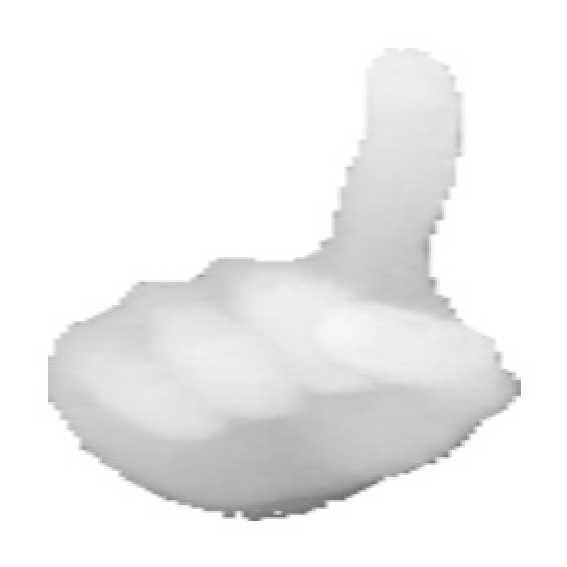
\includegraphics[width=.075\textwidth]{img/S01num1.eps} 
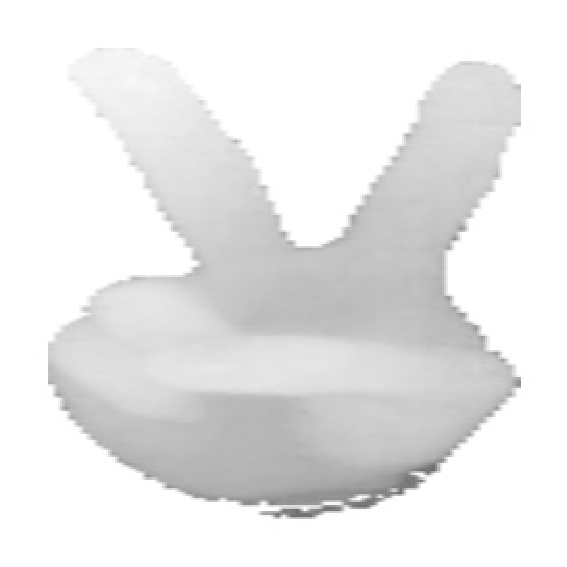
\includegraphics[width=.075\textwidth]{img/S01num2.eps}
$\cdots$ 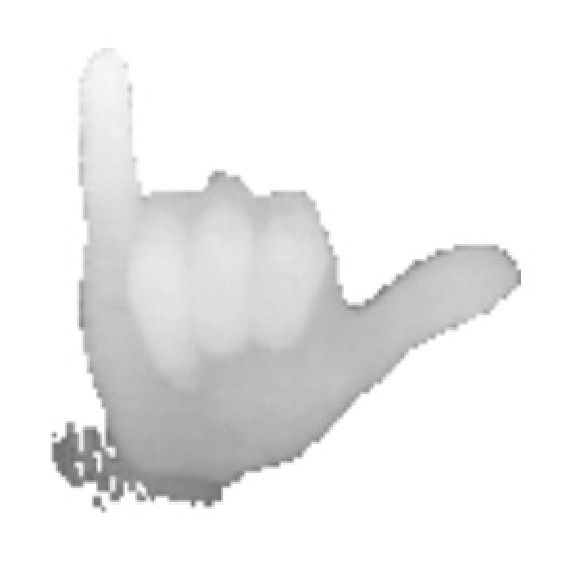
\includegraphics[width=.075\textwidth]{img/S01num31.eps}};

\node[] at ([xshift=4pt,yshift=-1pt]lowermiddle) {$\ldots$};

\draw[arr,draw=black] (cuadramiddle) to (lowermiddle);
\draw[arr,<->] (lowermiddle) to (lowerMiddleDec) ;
\draw[arr,<->] (middle) to (middleDec);
\draw[arr,draw=black] 
  (upper) -- 
  ++(0pt,1cm) node[above] {predicted class};
\draw[arr,dashed,draw=black] 
  (lowermiddle) to[out=45,in=315] (middle);
\draw[arr,dashed,draw=black] 
  (middle) to[out=45,in=315] (upper);


\node[anchor=north west,align=left] 
  at (upper) {\hspace{0.7in} neural network layer}; 
\node[anchor=north west,align=left] 
  at (middleDec) {\\ \hspace{0.7in} decoding layer}; 
\node[anchor=north west,align=left] 
  at (middle) {\hspace{0.7in} encoding layer}; 
\node[anchor=north west,align=left] 
  at (lowerMiddleDec) {\\ \hspace{0.7in} decoding layer}; 
\node[anchor=north west,align=left] 
  at (lowermiddle) {\\ \hspace{0.7in} encoding layer}; 
\end{tikzpicture}
\caption{Deep architecture during training. The training begins with the first
two layers, encoder - decoder, and once the training is complete feature are
encoded and propagated to the third layer in order to further
encode - decode high-level features. Finally, the last neural layer retrieves
the encoded features from the third layer and learns the target class. The
training is performed using SCG descent \cite{le2013building}.}
\label{fig:TrainingArchitecture}
\end{figure}
The first two layers are a set of unsupervised autoencoders that minimize the
loss function in (\ref{eq:loss}). The first layer, i.e., an encoding layer,
receives as input $N$ images of $256\times 256$ as row vectors, each denoted as 
$\mathbf{x}_n \in \mathbb{R}^{65536}$, where $n \in \{1,2, \dots, N\}$. The
training phase encodes the attibutes using 100 neural units to produce
$\mathbf{\hat{x}}_n \in \mathbb{R}^{100}$, and decodes back to
the feature space using, intuitively, 65536 neural units; all neural units use
logistic activation functions. 

Similarly, the third and fourth layers are an encoder and decoder,
respectively. The encoder in the third layer receives as input an encoded
version of the input coming from the first layer, denoted as
$\mathbf{\hat{x}}_n$, and encodes using 50 neural units producing a modified
version of the feature vector denoted as 
$\mathbf{\tilde{x}}_i \in \mathbb{R}^{50}$. 
The decoder in the fourth layer decodes using 100 neural units. 

In the last layer of the model we use a network of 31 neural units with softmax
activation functions. Each neuron is estimulated $\mathbf{\tilde{x}}_n$ and is
trained to predict the probability of the $n$-th sample belonging to a specific
class $C \in \{1, 2, \dots, 31\}$. The output of this layer for the $n$-th
sample is the estimated probability of that sample belonging to all classes, 
formally denoted as $\mathbf{\hat{d}}_n \in \mathbb{R}^{31}$. The layer is trained to minimize
the cross entropy function \cite{szegedy2016rethinking} given by:
\begin{align}
E=\frac{1}{N} \sum_{n=1}^N \sum_{c \in C} \hat{d}_{cn} \ln d_{cn} + (1 -
\hat{d}_{cn}) \ln (1 - d_{cn}) 
\label{eq:entropy}
\end{align}
where $\mathbf{d}_n \in \mathbb{R}^{31}$ is the true probability of the $n$-th
sample belonging to a specific class. 

Once the process of training the autoencoders and the softmax layer, the
network undergoes a last refined training phase. In this last process, only the
first, third, and fifth layers are fully connected and trained simmulating a
feed-forward neural network, as shown in Figure \ref{fig:finalArchitecture}. 
\begin{figure}
\centering
\begin{tikzpicture}[node distance=1.5cm and 1.25cm]
\node[redondo=2cm,label={120:\emph{softmax} activations}]
  (upper)
  {};
\pic at (upper.west) {dosp};
\pic at ([xshift=-0.75cm]upper.east) {unop};
\node[] 
  at ([xshift=4pt,yshift=-1pt]$ (upper.center) $ ) {$\ldots$};

\node[redondo=3.3cm,below=of upper,label={140:\emph{logistic} activations}]
  (middle)
  {};
\pic at (middle.west) {tresp};
\pic at ([xshift=-1.04cm]middle) {dosp};
\pic at ([xshift=-0.75cm]middle.east) {dosp};
\node[] at ([xshift=4pt,yshift=-1pt]middle) {$\ldots$};

\node[redondo=6.4cm,below=of
middle,label={140:\emph{logistic} activations}]
  (lowermiddle)
  {};
\pic at (lowermiddle.west) {tresp};
\pic at ([xshift=-1.85cm]lowermiddle) {tresp};
\pic at ([xshift=-2.58cm]lowermiddle) {tresp};
\pic at ([xshift=-1cm]lowermiddle.east) {tresp};
\node[cuadra,below=of lowermiddle,label={right:{input image}}] (cuadramiddle)
{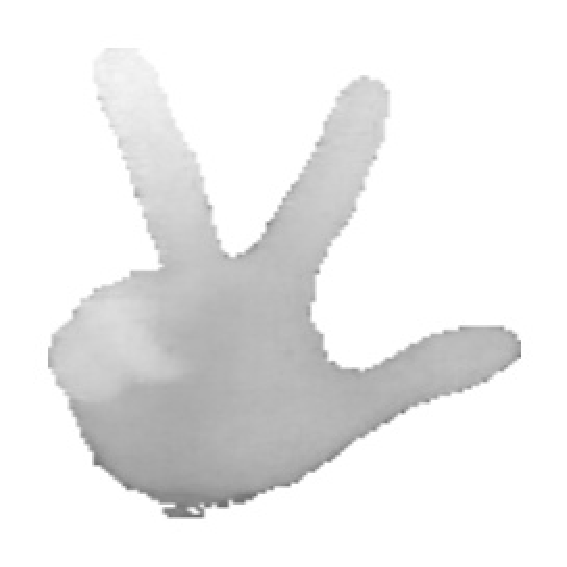
\includegraphics[width=.075\textwidth]{img/S01num3.eps}};

\node[] at ([xshift=4pt,yshift=-1pt]lowermiddle) {$\ldots$};

\draw[arr] (cuadramiddle) -- ++(0pt,1.5cm) node[above] {$\mathbf{x}_{n} \in \mathbb{N}_+^{65536}$};
\draw[arr] (lowermiddle) -- ++(0pt,1cm) node[above] {$\mathbf{\hat{x}}_n \in \mathbb{R}_+^{100}$};
\draw[arr] (middle) -- ++(0pt,1cm) node[above] {$\mathbf{\tilde{x}}_n \in \mathbb{R}_+^{50}$};
\draw[arr] 
  (upper) -- 
  ++(0pt,1cm) node[above] {output $\mathbf{d}_n \in \mathbb{R}_+^{31}$};
\node[anchor=north west,align=left] 
  at (upper) {\hspace{0.7in} neural network layer}; 
\node[anchor=north west,align=left] 
  at (middle) {\hspace{0.7in} sparse encoding layer}; 
\node[anchor=north west,align=left] 
  at (lowermiddle) {\\ \hspace{0.7in} sparse encoding layer}; 
\end{tikzpicture}
\caption{The working architecture when testing the system. The input is any
test image which is passed through the first sparse encoder in the stack,
reducing the dimensionality of the problem to 100. In the second sparse encoder
the feature space is further reduced to 50. The output are probabilistic
outputs corresponding to each of the 31 classes.}
\label{fig:finalArchitecture}
\end{figure}
The initial weights are those obtained during the
encoding-decoding learning phase and fine tuned using SCG descent to minimize
the cross entropy in (\ref{eq:entropy}).


\section{Experiments}
\subsection{Setup}
\subsection{Results and Discussion}

\bibliographystyle{splncs03} 
\bibliography{ref}
\end{document}
